\documentclass[a4paper]{article}
\usepackage[margin=1.5cm]{geometry} % Change the margins
\usepackage[utf8]{inputenc} % - Defines what coding LaTeX uses. Use this one.
\usepackage[english]{babel}
\usepackage[T1]{fontenc}
\usepackage{graphicx} % - Package for including images in the document.
\usepackage{amsmath}
\usepackage{amssymb}
\usepackage{mathtools}
\usepackage{listings}
\usepackage{textgreek}
\usepackage{caption} % Correct spacing for captions
\usepackage{siunitx} % Package for handling numbers (ex \num{1e6}), units (ex \SI{15,3}{Nm}) and intervals (ex \SIrange{10}{20}{\celcius}) correctly
\sisetup{output-decimal-marker={,},range-phrase=--,range-units=single,exponent-product=\cdot} % If you write in English, remove output-marker...
\graphicspath{ {Images/} } % - Path to where the images are located on your computer. In this case I have a folder (look to the left) "Images" where the images are gathered.
\usepackage{hyperref} % - Package for including hyperlinks in the document.
\usepackage[style=apa,backend=biber]{biblatex} % APA-referenser
\usepackage{mhchem}
\DeclareLanguageMapping{swedish}{swedish-apa}  % APA-referenser
 % - Package for the bibliography ("referenser").
\addbibresource{references.bib} % - From where, i.e. which file, the references are taken. The bibliography file is called name.bib; see left column.

\title{Lab 2}

\author{
Author \\
{Klas Mannberg,   klaman-8@student.ltu.se
} \\ \\

\includegraphics[width=0.2\textwidth]{ltu_swe.jpg}}
\date{12 May 2020}

\begin{document}

\maketitle

\section{Assignments}
\subsection{Assignment 1}
For $z=a+bi$  and its conjugate $z=a-bi$ the values of $a$ and $b$ are the same. This means the conjugate will also be on our complex plane only with a flipped axis of the imaginary axis. This means the conjugate is within the unit circle and is a defined singularity. 


\subsection{Assignment 2}
The system is casual when I add one additional singularity, a pole within our plane say at $z=0$. See figure \ref{fig:1}

\begin{figure}
    \centering
    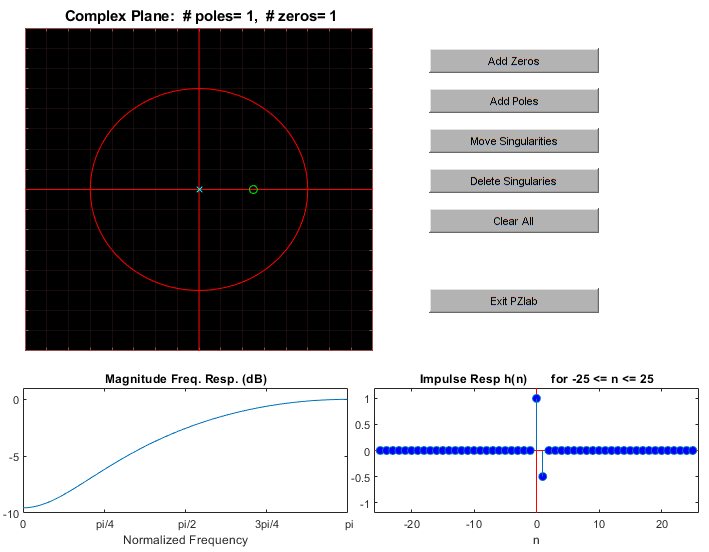
\includegraphics{1.png}
    \caption{Assignment 2}
    \label{fig:1}
\end{figure}
\subsection{Assignment 3}
The frequency response null area becomes more precise and focused at one point. See figure \ref{fig:2}

\begin{figure}
    \centering
    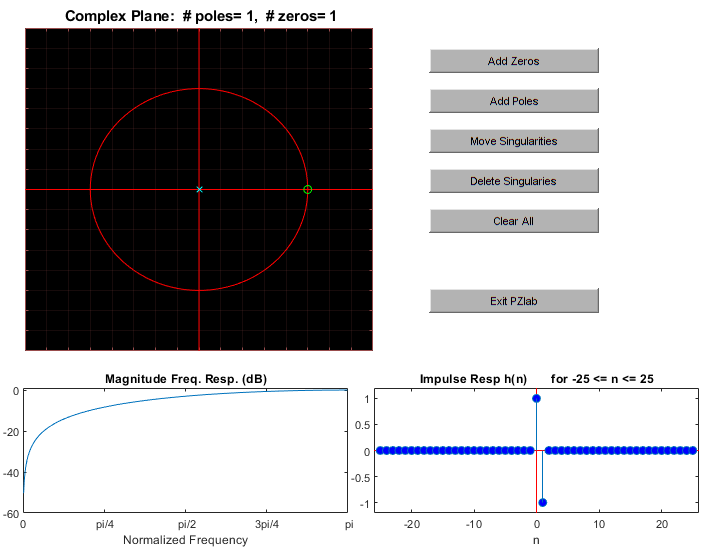
\includegraphics{2.png}
    \caption{Assignment 3}
    \label{fig:2}
\end{figure}
\subsection{Assignment 4}
The frequency at which the null appears gets shifted positively.See figure \ref{fig:3}

\begin{figure}
    \centering
    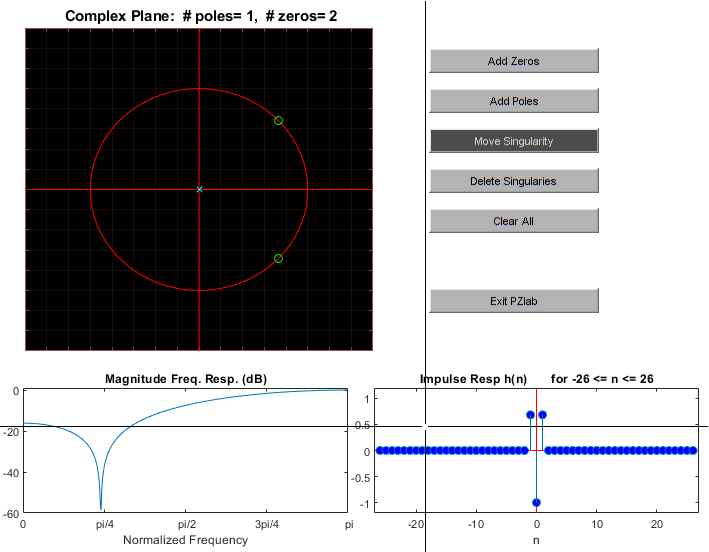
\includegraphics{3.png}
    \caption{Assignment 4}
    \label{fig:3}
\end{figure}
\subsection{Assignment 5}
1. This looks casual already. See figure \ref{fig:4} \\
2. The response becomes broad and covers a larger and larger range of frequencies. See figure \ref{fig:5}\\
3. The frequency for the small part that is not nulled gets shifted positively.See figure \ref{fig:6}
\begin{figure}
    \centering
    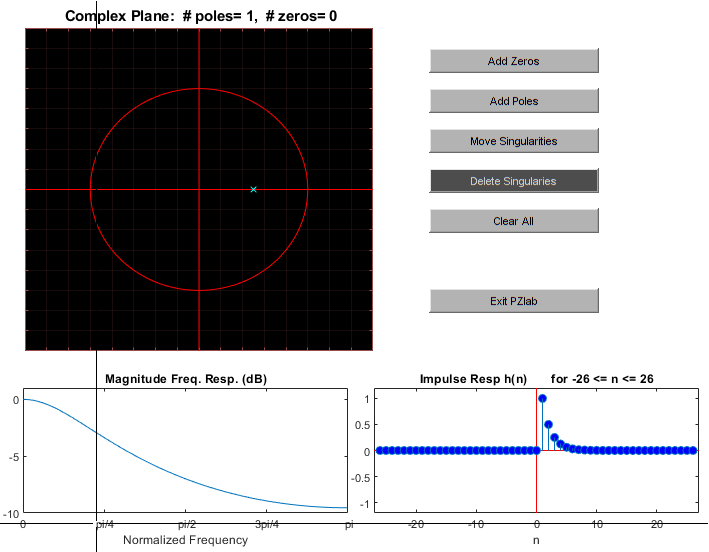
\includegraphics{4.png}
    \caption{Assignment 5.1}
    \label{fig:4}
\end{figure}
\begin{figure}
    \centering
    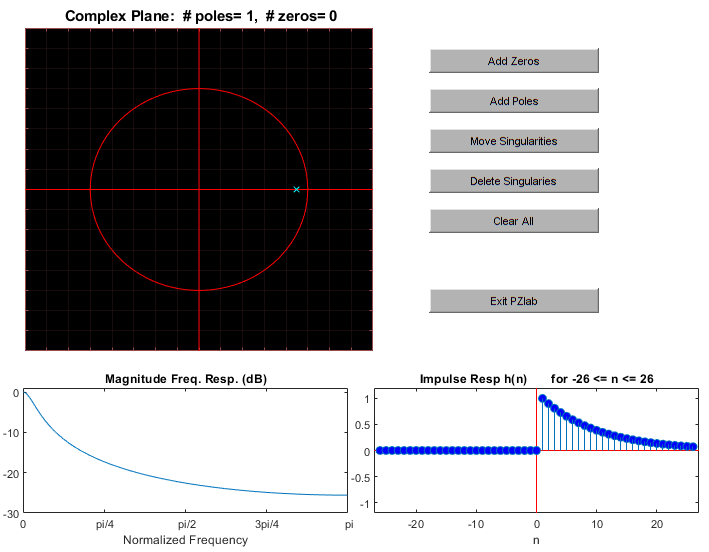
\includegraphics{5.png}
    \caption{Assignment 5.2}
    \label{fig:5}
\end{figure}
\begin{figure}
    \centering
    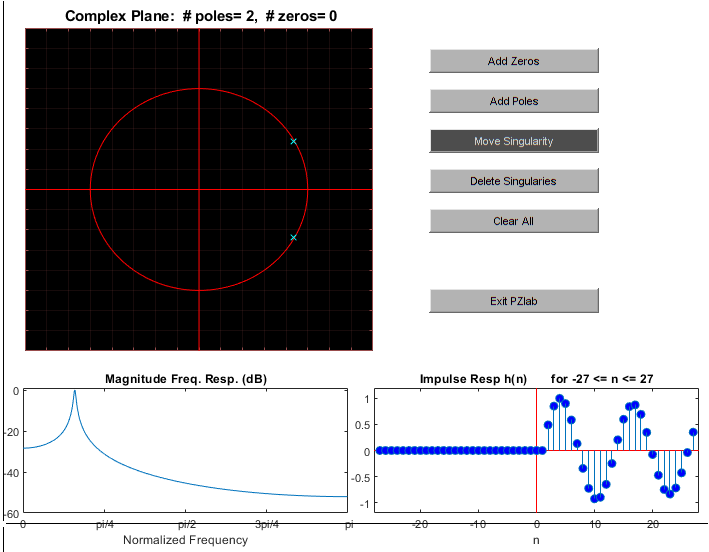
\includegraphics{6.png}
    \caption{Assignment 5.3}
    \label{fig:6}
\end{figure}
\subsection{Assignment 6}
The locations of the singularities seems to have direct effect to the nulling target frequencies and the range of frequencies the null covers.
\subsection{Assignment 7}
Placing a zero at $\frac{pi}{4}$ , which is our root $z_1 = 1e^{j\frac{\pi}{4}}$ gives us a null at that location, see figure \ref{fig:7}.  \\
We have values in the finite interval $-2 \leq n \leq 0$ with the values $\{h[-2],h[-1],h[0]\} = \{\sim0.71,-1,\sim0.71\}$ \\ $\therefore \{B_k\} = \{\sim0.71,-1,\sim0.71\}$ for k $= \{-2,-1,0\} \implies y[n] = 0.71x[n+2]-1x[n+1]+ 0.71x[n-0]$ 
\begin{figure}
    \centering
    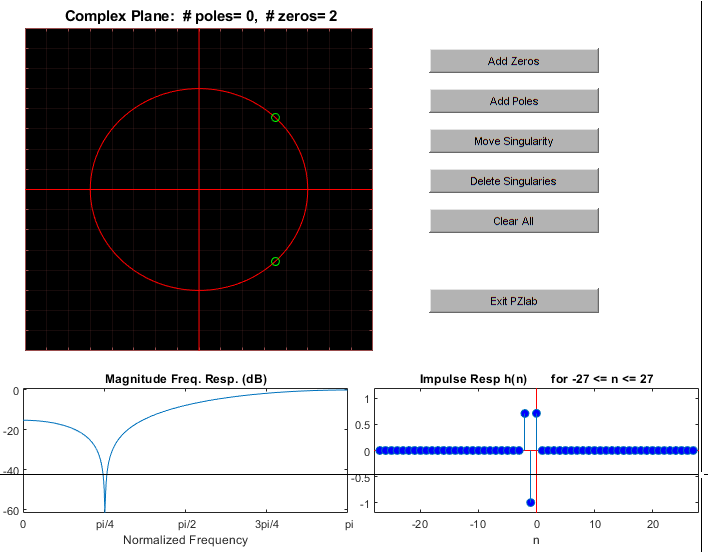
\includegraphics{7.png}
    \caption{Assignment 7}
    \label{fig:7}
\end{figure}
\subsection{Assignment 8}
Adding two poles next to the target zero refines the null input to be alot more precise. To flatten out the rest of the frequencies we add poles around the plane. The more poles I insert all round to negate the zero the better. The following figure could be improved a lot with even more poles. See figure \ref{fig:8}\\
\begin{figure}
	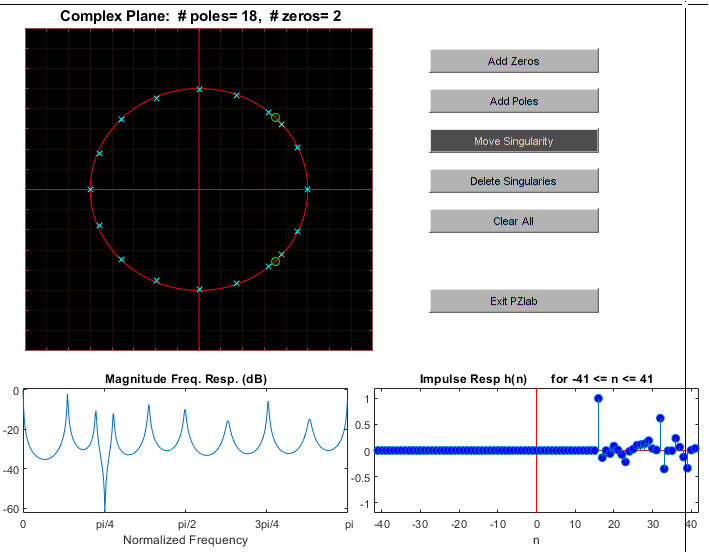
\includegraphics{assignment8.png}
	\caption{Assignment 8-\textit{Yes my windows makes the backround black which makes placing the singularities very hard}}
	\label{fig:8}
\end{figure}
\subsection{Assignment 9}
Got this to work with the command audioread with the following code block:
\begin{lstlisting}
function assign9 = assign9()
    load PZoutput;
    [audio,FS] = audioread('black.wav');
    result = filter(real(pz_poles),real(pz_zeros),audio);
    sound(result,FS);
\end{lstlisting}
And using zeros, and poles as shown in figure \ref{fig:9} \\
\begin{figure}
	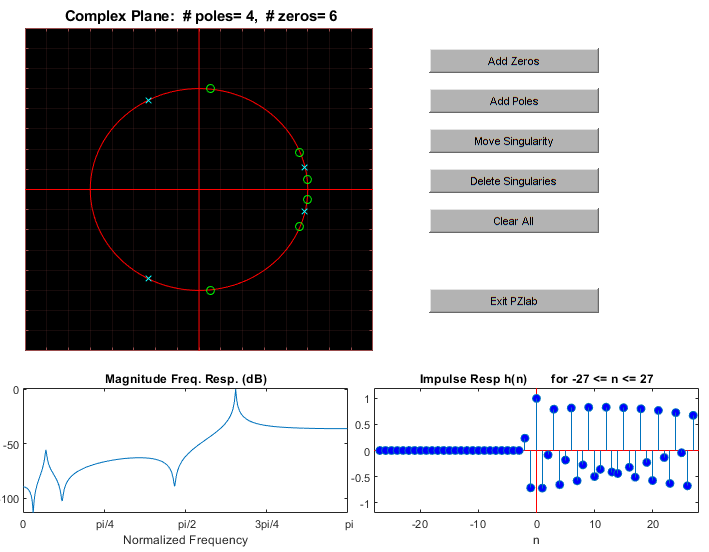
\includegraphics{9.png}
	\caption{Assignment 9}
	\label{fig:9}
\end{figure}
After the filter the music sounds raspier and lower quality. 
\end{document}
